%% This template can be used to write a paper for
%% Computer Physics Communications using LaTeX.
%% For authors who want to write a computer program description,
%% an example Program Summary is included that only has to be
%% completed and which will give the correct layout in the
%% preprint and the journal.
%% The `elsarticle' style is used and more information on this style
%% can be found at 
%% http://www.elsevier.com/wps/find/authorsview.authors/elsarticle.
%%
%%
\documentclass[preprint,12pt]{elsarticle}

%% Use the option review to obtain double line spacing
%% \documentclass[preprint,review,12pt]{elsarticle}

%% Use the options 1p,twocolumn; 3p; 3p,twocolumn; 5p; or 5p,twocolumn
%% for a journal layout:
%% \documentclass[final,1p,times]{elsarticle}
%% \documentclass[final,1p,times,twocolumn]{elsarticle}
%% \documentclass[final,3p,times]{elsarticle}
%% \documentclass[final,3p,times,twocolumn]{elsarticle}
%% \documentclass[final,5p,times]{elsarticle}
%% \documentclass[final,5p,times,twocolumn]{elsarticle}

%% if you use PostScript figures in your article
%% use the graphics package for simple commands
%% \usepackage{graphics}
%% or use the graphicx package for more complicated commands
%% \usepackage{graphicx}
%% or use the epsfig package if you prefer to use the old commands
%% \usepackage{epsfig}

%% The amssymb package provides various useful mathematical symbols
\usepackage{amssymb}
%% The amsthm package provides extended theorem environments
%% \usepackage{amsthm}

%% The lineno packages adds line numbers. Start line numbering with
%% \begin{linenumbers}, end it with \end{linenumbers}. Or switch it on
%% for the whole article with \linenumbers after \end{frontmatter}.
%% \usepackage{lineno}

%% natbib.sty is loaded by default. However, natbib options can be
%% provided with \biboptions{...} command. Following options are
%% valid:

%%   round  -  round parentheses are used (default)
%%   square -  square brackets are used   [option]
%%   curly  -  curly braces are used      {option}
%%   angle  -  angle brackets are used    <option>
%%   semicolon  -  multiple citations separated by semi-colon
%%   colon  - same as semicolon, an earlier confusion
%%   comma  -  separated by comma
%%   numbers-  selects numerical citations
%%   super  -  numerical citations as superscripts
%%   sort   -  sorts multiple citations according to order in ref. list
%%   sort&compress   -  like sort, but also compresses numerical citations
%%   compress - compresses without sorting
%%
%% \biboptions{comma,round}

% \biboptions{}

%% This list environment is used for the references in the
%% Program Summary
%%
\usepackage{lineno}
\usepackage{amsmath}
\usepackage{float}
\usepackage[version=4]{mhchem}
\usepackage{booktabs}
\usepackage{siunitx}
\usepackage{bm}

\restylefloat{table}

\usepackage{hyperref}

\newcommand{\BS}{\boldsymbol}

\newcounter{bla}
\newenvironment{refnummer}{%
\list{[\arabic{bla}]}%
{\usecounter{bla}%
 \setlength{\itemindent}{0pt}%
 \setlength{\topsep}{0pt}%
 \setlength{\itemsep}{0pt}%
 \setlength{\labelsep}{2pt}%
 \setlength{\listparindent}{0pt}%
 \settowidth{\labelwidth}{[9]}%
 \setlength{\leftmargin}{\labelwidth}%
 \addtolength{\leftmargin}{\labelsep}%
 \setlength{\rightmargin}{0pt}}}
 {\endlist}

\journal{Computer Physics Communications}

\begin{document}

\begin{frontmatter}

%% Title, authors and addresses

%% use the tnoteref command within \title for footnotes;
%% use the tnotetext command for the associated footnote;
%% use the fnref command within \author or \address for footnotes;
%% use the fntext command for the associated footnote;
%% use the corref command within \author for corresponding author footnotes;
%% use the cortext command for the associated footnote;
%% use the ead command for the email address,
%% and the form \ead[url] for the home page:
%%
%% \title{Title\tnoteref{label1}}
%% \tnotetext[label1]{}
%% \author{Name\corref{cor1}\fnref{label2}}
%% \ead{email address}
%% \ead[url]{home page}
%% \fntext[label2]{}
%% \cortext[cor1]{}
%% \address{Address\fnref{label3}}
%% \fntext[label3]{}

\title{RadLib: a radiative heat transfer model library for CFD}

%% use optional labels to link authors explicitly to addresses:
%% \author[label1,label2]{<author name>}
%% \address[label1]{<address>}
%% \address[label2]{<address>}

%\author[a]{First Author\corref{author}}
%\author[a,b]{Second Author}
%\author[b]{Third Author}

%\cortext[author] {Corresponding author.\\\textit{E-mail address:} firstAuthor@somewhere.edu}
%\address[a]{First Address}
%\address[b]{Second Address}

\author{Victoria B. Stephens}
\author{Sally Jensen}
\author{Isaac Wheeler}
\author{David O. Lignell\corref{cor1}}

\cortext[cor1]{Corresponding author. \ead{davidlignell@byu.edu}}

\address{Department of Chemical Engineering, Brigham Young University, Provo, UT 84602, United States}

\begin{abstract}
RadLib is a modular C++ library of radiation property models that can be applied to variety of systems involving radiative heat transfer, including CFD simulations. RadLib includes three major radiation property models---Planck Mean (PM) absorption coefficients, the weighted sum of gray gases (WSGG) model, and the rank-correlation spectral line weighted-sum-of-gray-gases (RCSLW) model---but its modular design and C++ and Python interface options permit convenient expansion to additional models. Several example cases illustrate the use of the models with an included ray-tracing solver and compare them in terms of accuracy relative to line-by-line solutions. The computational cost of the models is also compared. RadLib provides researchers with convenient access to validated radiation property models and a framework for further development. 
\end{abstract}


%In addition to the manuscript you must supply: the program source code; a README file giving the names and a brief description of the files/directory structure that make up the package and clear instructions on the installation and execution of the program; sample input and output data for at least one comprehensive test run; and, where appropriate, a user manual.

%A compressed archive program file or files, containing these items, should be uploaded at the "Attach Files" stage of the EM submission.

%For files larger than 1Gb, if difficulties are encountered during upload the author should contact the Technical Editor at cpc.mendeley@gmail.com.


\begin{keyword}
radiative heat transfer \sep reacting flows  \sep CFD \sep WSGG \sep RCSLW
\end{keyword}

\end{frontmatter}

\linenumbers

% PROGRAM SUMMARY.

{\bf PROGRAM SUMMARY}
  %Delete as appropriate.

\begin{small}
\noindent
{\em Program Title:} RadLib                                         \\
{\em CPC Library link to program files:} (to be added by Technical Editor) \\
{\em Developer's repository link:} https://github.com/BYUignite/radlib \\
{\em Code Ocean capsule:} https://codeocean.com/capsule/0997975/tree \\
{\em Licensing provisions(please choose one):} MIT \\
{\em Programming language:} C++, Python                                   \\
{\em Nature of problem(approx. 50-250 words):} \\
Radiation property models can be difficult to understand and implement, often requiring a high degree of specialization. This presents a problem for practitioners who wish to use/implement radiation models for which such models consitute only a small but important part of a larger simulation. Turbulent combustion simulations are one such example. Often, rudimentary assumptions are made and this can negatively impact results. \\
{\em Solution method(approx. 50-250 words):}\\
We provide a well-written, documented, and validated radiation property library that is open source, and uses modern versioning build tools. C++ and Python interfaces are provided along with several examples demonstrating usage of the model. The library can be extended to other models and interfaces. \\ 
{\em Additional comments including restrictions and unusual features (approx. 50-250 words):}\\
The library is intended to be used in Linux-like terminal applications.  
   \\

\end{small}

%%%%%%%%%%%%%%%%%%%%%%%%%%%%%%%%%%%%%%%%%%%%%%%%%%%%%%%%%%%%%%%%%%%%%%%%%%%%%%%%

\section{Introduction} \label{s:motivation}

Modeling radiative heat transfer for CFD is complex and challenging. Combustion simulations, for example, which require many physics models, are often complicated by the need for accurate radiation modeling, which can be difficult to implement and computationally expensive relative to simulation cost. This can lead to simulations that use oversimplified radiation models, but in cases where radiation is significant relative to the other physical phenomena, oversimplified models can negatively impact the accuracy of simulation results. In some cases, radiative gains or losses are small compared to other energy sources or heat transfer modes and radiation can be safely neglected, but many practical engineering systems do not allow this. For example, simple jet flames demonstrate both possibilities: early in a flame's development, turbulent mixing typically dominates heat transfer and dictates flame behavior; late-stage flame phenomena like soot behavior and flame sheet breakthrough, however, increasingly depend on the magnitude of radiative heat losses and are difficult to simulate accurately without a robust radiation model. These problems motivated development of the RadLib library, which provides a framework and uniform interface for radiation property models and implements three powerful models in C++ and Python, giving researchers more convenient access to advanced radiation property models and a consistent framework for further model development. 

The core mechanisms of radiative phenomena are physically and mathematically complex. Unlike other modes of heat transfer, radiation is governed by a set of integro-differential equations that depend on both direction and wavelength, known as the radiative transfer equations (RTE). Solving the RTE for a given system also requires information about the radiative properties of the materials and media involved, typically radiation absorption coefficients. These absorption coefficients are dependent on a number of local system properties such as temperature, pressure, and gas composition. As a result, computational radiation solvers require two parts: first, a solution approach for the radiative transfer equations (RTE); and second, a radiation property model. RadLib addresses the second part by providing a set of implemented and validated radiation property models that can be applied to various solution approaches for the RTE.

%Like combustion, the core mechanisms of radiation are physically and mathematically complex. Unlike other modes of heat transfer, radiation is governed by a set of integro-differential equations that depend on both direction and wavelength. Only the simplest systems have analytic solutions, and most practical systems require a numerical solution. Ray tracing solutions are very accurate but extremely computationally expensive, and often require high-performance computing resources to execute. Modeling assumptions are common and can reduce simulation cost at the expense of accuracy, depending on their validity for the system in question. 

With RadLib, we provide a convenient, easy-to-use access point for radiative property models that can be interfaced with various RTE solution approaches suitable for CFD applications. RadLib is a modular C++ library with an optional Python interface used to compute the radiation properties of participating media, which can be a difficult and time-consuming portion of radiation calculations. RadLib's current focus is calculating radiation absorption coefficients and weighting factors for use in global radiation models, but the expansion to other radiative properties is possible. Three models are fully implemented and validated and use a common interface, allowing researchers convenient access to radiation modeling tools suitable for various applications.

%%%%%%%%%%%%%%%%%%%%%%%%%%%%%%%%%%%%%%%%%%%%%%%%%%%%%%%%%%%%%%%%%%%%%%%%%%%%%%%%%

\section{Model descriptions} \label{s:models}

The RTE for intensity $I$ in (unit) direction $\mathbf{s}$ for an absorbing, emitting, and non-scattering medium is described by
% 
\begin{linenomath}
\begin{equation} \label{e:RTE_general}
    \frac{dI_{\eta}}{ds} = -\kappa_{\eta}I_{\eta} + \kappa_{\eta}I_{b,\eta},
\end{equation}
\end{linenomath}
%
where $I_{\eta}$ is the radiative spectral intensity, 
$I_{b\eta}$ is spectral blackbody intensity (or Planck function), 
$\kappa_{\eta}$ is the spectral absorption coefficient of the medium, and $s$ is a path length along direction $\mathbf{s}$. Radiation property models such as those implemented by RadLib are used to calculate the absorption coefficients $\kappa_{\eta}$. 
%
The gas absorption spectrum is an extremely complex function consisting of millions of spectral lines (peaks) corresponding to quantum mechanical energy levels of the gas molecules.
Direct solution of Eq.~\ref{e:RTE_general}, involves so-called line-by-line calculations that are computationally prohibitive for most practical configurations and are used primarily for model validation. Global models are an important class of radiation property models that make use of spectrally-integrated radiation properties and are usually versions of the weighted sum of gray gases (WSGG) model \cite{Hottel_1967,Modest_2013}. For instance, integrating Eq.~\ref{e:RTE_general} over fixed spectral ranges $\eta_j$ and assuming gray (spectrally uniform) properties in each region $j$, (that is, in each gray gas $j$), gives
%
\begin{linenomath}
\begin{equation} \label{e:RTE_wsgg}
	\frac{dI_j}{ds} = -\kappa_jI_j + a_j\kappa_jI_b, \hspace{20pt} j=0,1,...,n,
\end{equation}
\end{linenomath}
%
where $a_j$ is a weight factor defined as
%
\begin{linenomath}
\begin{align}
    &a_j= \frac{\int_{\eta_j}I_{b,\eta}d\eta}{I_b},\\
    &\sum_j a_j = 1.
\end{align}
\end{linenomath}
%
Given spatial profiles of $\kappa_j$ and $a_j$, Eq.~\ref{e:RTE_wsgg} can be computed for each of the $n+1$ gray gases. Normally, the $j=0$ gas is considered as a clear gas and represents transparent windows in the spectrum for which $\kappa_0=0$.
The total radiative intensity $I$ is calculated by summing the individual gray gas intensities:
%
\begin{linenomath}
\begin{equation}
	I=\int_{\eta=0}^{\infty}I_{\eta}d\eta=\sum_{j=1}^n I_j.
\end{equation}
\end{linenomath}
%
Radiative intensity $I$ is a function of direction $\mathbf{s}$. The heat flux vector $\mathbf{q}$ is found by integrating over directional solid angles ($\mathbf{s}\Omega$) on the sphere:
%
\begin{linenomath}
\begin{equation}
    \mathbf{q} = \int_{4\pi}I(\mathbf{s})\mathbf{s}d\Omega.
\end{equation}
\end{linenomath}
%
The volumetric radiative heat source is then 
%
\begin{linenomath}
\begin{equation}
    Q = -\nabla\cdot\mathbf{q}.
\end{equation}
\end{linenomath}
%

RadLib currently implements three models of varying complexity and accuracy to calculate the radiation absorption coefficients $\kappa_j$ and their weight factors $a_j$ for each gas $j$. The absorption coefficients are typically calculated using correlations relating them local properties such as temperature, pressure, and composition. Correlations come from curve fits to high-resolution radiation property databases. At present, RadLib considers up to four gas species (H$_2$O, CO, CO$_2$, and CH$_4$) and soot. 

While solving the RTE is not the focus of this software, RadLib's example cases do employ a simple ray tracing solver to calculate the radiative heat flux and volumetric heat source profiles between two parallel planes. 

%[OTHER THINGS THAT APPLY TO ALL MODELS GO HERE]

%%%%%%%%%%%%%%%%%%%%%%%%%%%%%%%%%%%%%%%%%%%%%%%%%%%%%%%%%%%%%%%%%%%%%%%%%%%%%%%%

\subsection{Planck Mean absorption coefficients} \label{s:planckmean}

RadLib's simplest model uses Planck Mean absorption coefficients calculated from the correlations given on the TNF Workshop site \citep{Smith_2003}. The temperature-dependent correlations are based on the RADCAL model \citep{Grosshandler_1993}. The TNF radiation model is also documented in \citep{Barlow_2001}.

Planck Mean absorption coefficients are commonly used to model radiation, especially in combustion systems, because the model is relatively easy to implement, computationally inexpensive, and reasonably accurate in some cases. The Planck Mean model is most appropriate under optically thin conditions with relatively low radiative transfer relative to other heat sources such as reactive heat release rates. In cases where the optically thin assumption applies, such as simple hydrogen jet flames, this model and the associated Planck Mean absorption coefficients can produce accurate results \citep{Barlow_1999}. In cases where the optically thin assumption is not reasonable, including many other combustion scenarios, the Planck Mean model does not produce accurate results. For example, it significantly overpredicts radiative losses from the TNF library's CH$_4$ flames \cite{Frank_2000,Zhu_2002,Coelho_2002}. The examples included with the code and illustrated in Section \ref{s:Examples} demonstrate the deficiencies of the Planck Mean model in comparison to the others included with RadLib.

%%%%%%%%%%%%%%%%%%%%%%%%%%%%%%%%%%%%%%%%%%%%%%%%%%%%%%%%%%%%%%%%%%%%%%%%%%%%%%%%

\subsection{Weighted sum of gray gases (WSGG)} \label{s:wsgg}

The WSGG model was introduced in Sec.~\ref{s:models}.
RadLib implements the WSGG model presented by Bordbar et al. \citep{Bordbar_2014,Bordbar_2020}, which uses correlations based on the HITEMP 2010 database \cite{Rothman_2010}. It uses four gray gases and one transparent gas, and considers gaseous species \ce{CO2} and \ce{H2O}. This version of the WSGG model is advantageous because it allows for arbitrary \ce{CO2} and \ce{H2O} compositions, increasing its accuracy and flexibility. Absorption coefficients are calculated by 
%
\begin{linenomath}
\begin{equation}
    \kappa_j=\sum_{k=0}^{4}d_{j,k}M_r^k,
\end{equation}
\end{linenomath}
%
where $\kappa_j$ is the absorption coefficient for gray gas $j$, $d_{j,k}$ is a correlated model coefficient, and $M_r$ is the molar ratio $y_{\mathrm{H_2O}}/y_{\mathrm{CO_2}}$. The weight factors are calculated by 
%
\begin{linenomath}
\begin{equation}
    a_j=\sum_{k=0}^{4}b_{j,k}T_r^k,
\end{equation}
\end{linenomath}
%
where $a_j$ is the weighting factor for gas $j$ and $T_r$ is a scaled temperature equal to $T/T_{ref}$ with $T_{ref}=1200$K. The value of $b_{i,j}$ is calculated by 
%
\begin{linenomath}
\begin{equation}
 b_{j,k}=\sum_{i=0}^{4}C_{j,k,i}M_r^i,
\end{equation}
\end{linenomath}
%
where $C_{j,k,i}$ is another correlated model coefficient. The model coefficients $d_{j,k}$ and $C_{j,k,i}$ are provided by Bordbar et~al. \citep{Bordbar_2014,Bordbar_2020}. 

The correlations provided by Bordbar et~al. (2014) \cite{Bordbar_2014} are valid for $0.01\le M_r\le4$. In Bordbar et~al. (2020) \cite{Bordbar_2020} this range was extended to arbitrary $M_r$ by interpolating $\kappa_j$ and $a_j$ between the pure component values and the corresponding limit on $M_r$. That is, for \ce{CO2}, $\kappa_j$ and $a_j$ are interpolated between values at $M_r=0.01$ and pure \ce{CO2}; for \ce{H2O}, $\kappa_j$ and $a_j$ are interpolated between values at $M_r=4$ and pure \ce{H2O}.

%%%%%%%%%%%%%%%%%%%%%%%%%%%%%%%%%%%%%%%%%%%%%%%%%%%%%%%%%%%%%%%%%%%%%%%%%%%%%%%%

\subsection{Rank Correlated SLW (RCSLW)} \label{s:RCSLW}

The Spectral Line Weighted-Sum-of-Gray Gases (SLW) model represents a family of global approaches to radiative heat transfer in high-temperature gases that also includes Absorption Distribution Function (ADF) and Full Spectrum $k$-distribution (FSK) models, all of which are based on the same fundamental principle in modeling the gas absorption spectrum \cite{Solovjov_2016}. In order to extend their spectral models from uniform conditions (isothermal, homogeneous gases) to nonuniform conditions (non-isothermal, non-homogeneous gases), these models take a reference approach in which local gas states are corrected relative to a reference state. Reference approaches, however, generally lack consistent reference states and can yield significant errors in cases with large spatial temperature gradients \cite{Solovjov_2017}. The Rank Correlated SLW (RCSLW) model is a unique extension of the generalized SLW model that does not require a specified gas reference state and preserves the emission term of the spectrally integrated RTE. 
% TODO: what does this last phrase mean: preserves the emission...?
%
Recent comparison of advanced SLW modeling approaches revealed that ``the Rank Correlated SLW model is the most robust of all models, and demonstrates that it can achieve accurate solutions with as few as 3–5 gray gases" \citep{Badger_2019}. A brief overview of the RCSLW model is given here; detailed discussion can be found in the literature \cite{Solovjov_2000, Solovjov_2001, Solovjov_2008, Solovjov_2011, Solovjov_2014, Solovjov_2016, Solovjov_2017, Webb_2018}. 
In particular, Solovjov et~al. \cite{Solovjov_2017} present several RCSLW methods within a generalized framework; RadLib implements method I.2.2, which gives the best results and is summarized here.
%

SLW models are similar to WSGG models, but SLW gases are gray in a given band by construction, whereas in traditional WSGG approaches the gases are only conceptually gray, and the absorption coefficients and weights are determined empirically \cite{Badger_2019}. 
%
Instead of integrating within a sequential band of $\eta$ (with highly variable $\kappa$) to define a gray gas $j$ as in other WSGG models, SLW models perform their spectral integration over a set of nonsequential wavenumbers constituting a given band $j$ of absorption cross sections $C_\eta$.
%
The absorption coefficient is related to the absorption cross section by $\kappa_\eta=C_\eta N$, where $N$ is the molar density of the radiatively participating gas.
%
Using Solovjov's notation~\cite{Solovjov_2017}, $\Delta_j=\{\eta:\tilde{C}_{j-1}<C_\eta<\tilde{C}_j\}$ is the set of wavenumbers constituting gas $j$ in Eq.~\ref{e:RTE_wsgg}, where $\tilde{C}$ denotes a cross section boundary between two bands/gases.
%
Hence, in SLW models, the gases in a given band are gray to within the width $\tilde{C}_j-\tilde{C}_{j-1}$.

A gray gas weight $a_j$ is the fraction of blackbody emission from $\eta\in\Delta_j$ corresponding to a given cross-section band $j$. This weight $a_j$ is computed using the absorption line blackbody distribution function (ALBDF) \cite{Pearson_2014}, which gives the fraction of total blackbody emission from $\eta$ corresponding to absorption cross sections less than $C$: 
%
\begin{linenomath}
    \begin{equation} \label{e:albdf}
        F(C,\BS{\phi},T) = \frac{1}{\sigma T^4}\int_{\{\eta:\,C_\eta(\eta,\BS{\phi})<C\}}E_b(\eta,T)d\eta,
\end{equation}
\end{linenomath}
%
so that
%
\begin{linenomath}
    \begin{equation}\label{e:aj}
    a_j = F(\tilde{C}_j,\BS{\phi}, T) - F(\tilde{C}_{j-1}, \BS{\phi},T).
\end{equation}
\end{linenomath}
%
%todo: deal with T versus Tb in e:albdf and previous eqn.
Note that $F$ varies between zero and one, and is monotonic in $C$, allowing calculation of the inverse $C(F,\BS{\phi},T)$.

The WSGG RTE in Eq.~\ref{e:RTE_wsgg} assumes the sets $\Delta_j$ are independent of spatial position $\mathbf{x}$, but care must be taken since $C_\eta$ depends on the thermodynamic state (denoted by vector $\BS{\phi}$ with nominal components $T$, $P$, and $y_i$), which does vary spatially. That is, $C_\eta=C_\eta(\eta,\BS{\phi}(\mathbf{x}))$. Hence, spatially-fixed $\Delta_j$ with spatially varying $\BS{\phi}$ implies a spatial variation in $C_j$ and $\tilde{C}_j$.
 
The RCSLW model uses the notion of rank correlation to compute this variation in $C_j$ and $\tilde{C}_j$. 
Consider two positions with thermodynamic states $\BS{\phi}_1$ and $\BS{\phi}_2$. These will have corresponding spectra $C_\eta(\eta,\BS{\phi}_1)$, and $C_\eta(\eta,\BS{\phi}_2)$.
Now, let $\hat{C}_1\equiv C_\eta(\hat{\eta},\BS{\phi}_1)$ and $\hat{C}_2\equiv C_\eta(\hat{\eta},\BS{\phi}_2)$ denote the cross sections at some wavenumber $\hat{\eta}$. For each of the two spectra, we can define the set of wavenumbers that give cross sections less than $\hat{C}$:
%
\begin{linenomath}
\begin{align}
    H_1&=\{\eta: C_\eta(\eta,\BS{\phi}_1)<\hat{C}_1\}, \\
    H_2&=\{\eta: C_\eta(\eta,\BS{\phi}_2)<\hat{C}_2\}.
    \end{align}
\end{linenomath}
%
If $H_1=H_2$ for arbitrary $\hat{\eta}$, the spectra corresponding to $\BS{\phi}_1$ and $\BS{\phi}_2$ are said to be rank correlated.
% Solovjov provides some visual representations...

This rank correlation is used as follows. Consider Eq.~\ref{e:albdf} evaluated at $C=\hat{C}_1$, $\BS{\phi}=\BS{\phi}_1$, $T=T_r$, and again at
$C=\hat{C}_2$, $\BS{\phi}=\BS{\phi}_2$, $T=T_r$, where $T_r$ is some reference temperature:
%
\begin{linenomath}
    \begin{align} \label{e:albdf2}
        F(\hat{C}_1,\BS{\phi}_1,T_r) &= \frac{1}{\sigma T_r^4}\int_{H_1}E_b(\eta,T_r)d\eta, \\
        F(\hat{C}_2,\BS{\phi}_2,T_r) &= \frac{1}{\sigma T_r^4}\int_{H_2}E_b(\eta,T_r)d\eta.
    \end{align}
\end{linenomath}
%
Since $H_1=H_2$, we have 
%
\begin{linenomath}
    \begin{equation}\label{e:FeqF}
    F(\hat{C}_1,\BS{\phi}_1,T_r)=F(\hat{C}_2,\BS{\phi}_2,T_r).
\end{equation}
\end{linenomath}
%
Recall that $F$ can be inverted, so if $\hat{C}_1$ and $\BS{\phi}_1$ are given, we can compute $F$ and then invert to obtain $\hat{C}_2$ at $\BS{\phi}_2$. Now, note that Eq.~\ref{e:FeqF} is assumed to hold for arbitrary states $\BS{\phi}_1$ and $\BS{\phi}_2$; hence, if some $F$ is given or specified, we can invert $F=F(\hat{C},\BS{\phi},T_r)$ to get $\hat{C}$ at corresponding state $\BS{\phi}$. At this point, we can drop the \emph{hat} notation and just write $F(C,\BS{\phi},T_r)$.

Given the above summary development, the RCSLW model is applied as follows. 
%
\begin{enumerate}
    \item A reference temperature is specified. This is taken to be the average temperature on the domain of interest in \cite{Solovjov_2001}.
    \item A collection of $\tilde{F}_j$ values are specified, with $F_j$ points between $\tilde{F}_j$ and $\tilde{F}_{j-1}$. These apply to all spatial positions. 
    \item The corresponding $\tilde{C}_j$ and $C_j$ values at any spatial position and corresponding thermodynamic state $\BS{\phi}$ are found by inversion: $C_j = C(F_j,\BS{\phi},T_r)$, and $\tilde{C}_j = C(\tilde{F}_j,\BS{\phi},T_r)$
    \item $\kappa_j$ is then computed as $\kappa_j=C_jN$. 
    \item $a_j$ is computed from Eq.~\ref{e:aj}, where $T$ is taken as the local temperature.
\end{enumerate}
%

The ALBDF functions are provided by Pearson et~al.~\cite{Pearson_2014} for \ce{H2O}, \ce{CO2}, and \ce{CO} at pressures ranging from 0.1 to 50 atm, and temperatures from 300 to 3000 K in both tabulated and correlated form. The tabulated data are currently used in Radlib, coupled with multilinear interpolation. For gas mixtures, the multiplication method described in \cite{Solovjov_2000} is used, in which 
%
\begin{linenomath}
\begin{equation}
    F(C) = F_{CO2}(C/y_{CO2})F_{H2O}(C/y_{H2O})F_{CO}(C/y_{CO}), 
\end{equation}
\end{linenomath}
%
where the $\BS{\phi}$ and $T$ arguments of $F$ are omitted for clarity.

%%%%%%%%%%%%%%%%%%%%%%%%%%%%%%%%%%%%%%%%%%%%%%%%%%%%%%%%%%%%%%%%%%%%%%%%%%%%%%%%

\subsection{Soot} \label{s:soot}

RadLib can also account for the radiative properties of soot in combustion environments. Soot particles are assumed to be unagglomerated spheres that absorb and emit radiation at all wavelengths such that their optical properties can be determined using the Rayleigh small particle limit. Radiation scattering may be neglected because unagglomerated soot particles in the Rayleigh regime are still small relative to the wavelength of infrared radiation in flames \cite{Brewster_1992,Solovjov_2001}. The spectral soot absorption coefficient is given by 
%
\begin{linenomath}
\begin{equation}
\label{e:soot1}
	\kappa_{s,\eta}=C_0 f_v \eta, \; \; \; C_0 = \frac{36\pi n k}{(n^2-k^2+2)^2+4n^2k^2},
\end{equation}
\end{linenomath}
%
where $n$ and $k$ are the real and imaginary parts of the soot complex index of refraction, respectively, and $f_v$ is the soot volume fraction \cite{Solovjov_2001,Modest_2013}. Various values for the refraction index have been proposed and applied \cite{Lee_1981,Stull_1960,Dalzell_1969,Howarth_1966,Chang_1990,Felske_1984,Williams_2007}. 
% INSERT FIGURE SHOWING DIFFERENT MODELS
RadLib uses the values $n=1.75$ and $k=1.03$ given in \cite{Williams_2007}, which result in a value of $C_0=7.03$, which is nearly the same as the value $C_0=7.0$ used in \cite{Solovjov_2001}. 
The Planck mean and Rosseland mean soot absorption coefficients are given in \cite{Modest_2013} as $\kappa_s=3.83f_vC_0T/C_2$ and $\kappa_s=3.60f_vC_0T/C_2$, respectively.
Due to the small difference between the coefficients in these two expressions, a mean value is suggested \cite{Felske_1977,Modest_2013}:
%
\begin{linenomath}
\begin{equation}
\label{e:soot2}
	\kappa_{soot}=3.72\frac{f_vC_0T}{C_2},
\end{equation}
\end{linenomath}
%
where $T$ is the temperature and $C_2=0.014388$ \si{m.K} is a Planck function constant \cite{Modest_2013}. 

In the Planck Mean model, which treats a gas mixture as one gray gas, the soot absorption coefficient calculated from Eq.~\ref{e:soot2} is added to the gas absorption coefficient. This gives $\kappa_s=1817f_vT$ \si{m^{-1}}.
 
In the WSGG model, Bordbar suggested incorporating soot as follows \cite{Bordbar_personal}. The soot absorption coefficient is similarly calculated from Eq.~\ref{e:soot2} but is then added to each of the gases separately. Because soot radiates across all wavelengths, its absorption coefficient is added to the values of all four gray gases and the clear gas. The gas weights $a_j$ are not changed. This model yeilds the expected behavior in the soot-only and gas-only limits.

The soot model used in the WSGG model can be applied to the RCSLW model as well. However, the formulation of the RCSLW model allows for a spectral soot treatment in the same manner as the gas species~\cite{Solovjov_2001}. Calculation of the soot ALBDF is facilitated by the simple $\eta$ dependence of $\kappa_{s,\eta}$ in Eq.~\ref{e:soot1}. The fraction of the black energy at wavenumbers below $\eta$ is computed directly using a series expansion from Chang and Rhee \cite{Chang_1984,Solovjov_2001}. The soot ALBDF is then included in the product of species ALBDFs to obtain the mixture ALBDF. 
 
%%%%%%%%%%%%%%%%%%%%%%%%%%%%%%%%%%%%%%%%%%%%%%%%%%%%%%%%%%%%%%%%%%%%%%%%%%%%%%%%

\section{Software Description} \label{s:architechture}

RadLib is an object-oriented C++ class library that includes both C++ and Python interfaces. The RadLib package contains five subdirectories (upon initial download): \texttt{source} contains the RadLib source code; \texttt{build} contains installation files; \texttt{examples} contains instructive example cases, including a simple interface and solver for a parallel planes geometry; \texttt{data} contains ALBDF data tables required for the RCSLW model; and \texttt{docs} contains files used to generate code documentation with Doxygen (optional). 

The \texttt{source} and \texttt{examples} directories are further divided into \texttt{C++} and \texttt{Python} subdirectories to differentiate between interfaces. There are three interface options for using this code: C++, Python, and Cython-wrapped Python. C++ interfaces are located within the \texttt{examples/c++} folder, while Python interfaces are located within the \texttt{examples/python} folder. When running examples with Python, the Cython-wrapped version is the default; to run the regular Python version without the Cython wrapper, edit the comments near the top of the example files (i.e \texttt{ex\textunderscore S1.py}). The C++ interface produces the fastest-running code, followed by the Cython-wrapped Python interface and then the regular Python interface. [INSERT RUNTIME COMPARISONS HERE]

RadLib installation is automated with CMake. First, navigate to the \texttt{radlib/build} directory. If the user requires an installation location other than the default \texttt{radlib/installed} directory, edit the \texttt{user\textunderscore config} file before running CMake. To compile the package, run the command \texttt{cmake -C user\textunderscore config ../source}. Upon successful completion, run \texttt{make} and then \texttt{make install} to complete the process. The generated C++ library file is located at \texttt{radlib/installled/lib/libradlib.a}. 

Figure \ref{fig:flowchart} illustrates the basic structure use of the RadLib package within a generic example using the provided interfaces. The RadLib library generates absorption coefficients and their weighting factors for use within the appropriate RTE, but does not specify any particular geometry, making it a versatile tool for any simulation that requires radiative heat transfer, regardless of configuration. The interfaces, solver, and examples included with the library serve to illustrate its use and validate the implementation and results. 
%
\begin{figure}
	\begin{center}
        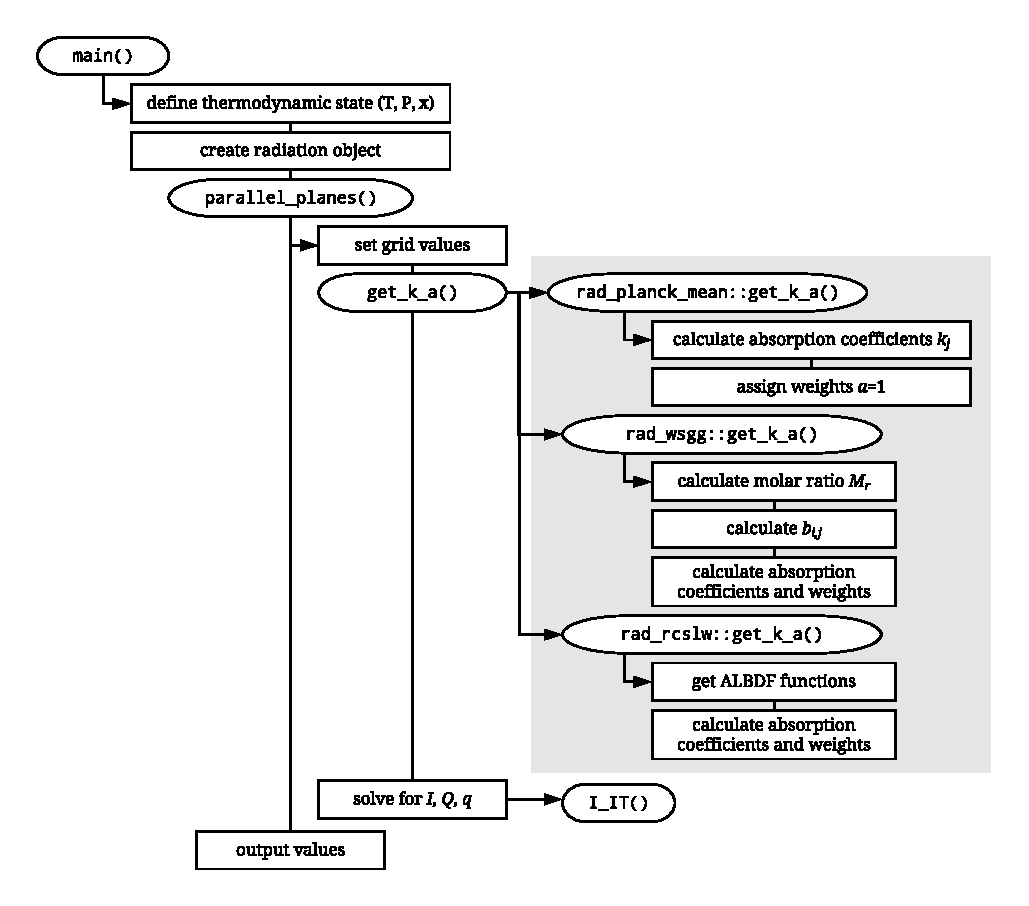
\includegraphics[width=\textwidth]{fig_radlib_structure.pdf}
	\end{center}
	\caption{Example workflow diagram. Highlighted areas are part of the RadLib library; other areas represent example infrastructure for using the package.}
\label{fig:flowchart}
\end{figure}
%

%%%%%%%%%%%%%%%%%%%%%%%%%%%%%%%%%%%%%%%%%%%%%%%%%%%%%%%%%%%%%%%%%%%%%%%%%%%%%%%%

\section{Validation and Examples} \label{s:Examples}

Several examples are presented to illustrate the behavior of the models. The examples show heat flux $q$ or volumetric heat source $Q$ in one one-dimensional configurations with varying gas compositions and temperatures. We compare the PM, WSGG, and RCSLW models for each example. The examples correspond to those presented by Solvojov et al. \cite{Solovjov_2017} (S), Bordbar et al. \cite{Bordbar_2020} (B), Solovjov et~al. \cite{Solovjov_2001} (Sb), and the number of each example corresponds to the example number in the respective reference. A ray-tracing code is used to solve the radiative transport equation between two parallel plates. 
Table~\ref{t:examples} summarizes the cases. Example S1 is a hot slab next to a cold slab where the cold slab's thickness varies; Example S2 is isothermal with a thick slab of high CO$_2$ next to a thin slab of low CO$_2$ with variable thickness; Example S3 uses parabolic temperature and H$_2$O mole fraction profiles; Example S4 has a triangular temperature profile between equally-spaced isothermal regions; Example S5 uses a half-sinusoid temperature profile that decreases from 1500 to 500 K; and Example B3 has symmetric temperature and H$_2$O mole fraction profiles with central peaks of 1800 K and 1, respectively (with $y_{CO2}=1-y_{H2O}$). Example Sb1 is a simple uniform temperature and composition profile with soot radiation. Each case is presented alongside the line-by-line (LBL) data presented in the references. 
%
\begin{table}
    \caption{Summary of example cases presented. S1-S5 are from \cite{Solovjov_2017}; B3 is from \cite{Bordbar_2020}; Sb1 is from \cite{Solovjov_2001}. All cases use $P=1$ atm and black walls.}
    \label{t:examples}
    \centering
    \resizebox{\textwidth}{!}{
    \begin{tabular}{c l l c c c}
        \hline
        Example & T(K)                           & $y_{H2O}$  $y_{CO2}$ (mole frac.)                     & L (m)   & $T_{walls}$ (K)\\
        \hline
        S1 & $T(x<0.5)=2000$; $T(x>0.5)=300$     & $y_{CO2}=0.1$, $y_{H2O}=0.2$                          & 0.5-2.5 & cold, cold     \\
        S2 & T=1000                              & $y_{CO2}(x<0.5)=0.4$, $y_{CO2}(x>0.5)=0.1$            & 0.5-2.5 & cold, cold     \\
           &                                     & $y_{H2O}=0.0$                                         &         &                \\
        S3 & $T(x) = 4000x(L-x)/L^2 + 800$       & $y_{H2O}(x) = 0.8x(L-x)/L^2 + 0.12$                   & 1       & 800, 800       \\
           &                                     & $y_{CO2}=0$                                           &         &                \\
        S4 & middle third triangular to 2500     & $y_{H2O}=0.1$, $y_{CO2}=0$                            & 0.3     & 500, 500       \\
        S5 & $T(x) = 1000 + 500\cos(\pi x/L)$    & $y_{H2O}=0.1$, $y_{CO2}=0$                            & 2       & 1500, 500      \\
        B3 & $T(x) = 400 + 1400\sin(\pi x/L)^2$  & $y_{H2O}(x) = 0.0001 + 0.9999\sin(\pi x/L)^2$         & 1       & 400, 400       \\
           &                                     & $y_{CO2}=1-y_{H2O}$                                   &         &                \\
        Sb1& $T = 1000$                          & $y_{H2O} = 0.2$, $y_{CO2}=0.1$, $y_{CO}=0.03$         & 1       & cold, cold     \\
        \hline
    \end{tabular}
    }
\end{table}
%
The examples are provided with the RadLib code and implemented in both C++ and Python. A Juptyer notebook is provided with the Python examples that runs the examples, displays the plots, and saves the plots to PDF files. Python and Cython versions of the one-dimensional solver \texttt{parallel\textunderscore planes.py} are provided for convenience. 

These cases are intended to illustrate the use of the RadLib library and are not exhaustive. Details about these examples and their motivations can be found in their respective references. While ommitted here for brevity, the implemented WSGG and RCSLW models give essentially identical results to those presented in \cite{Solovjov_2017,Bordbar_2020} such that these examples also serve as a validation of the implementation of the models.

Figure~\ref{f:examples} shows comparative results for the different radiation models for these cases. 
%
\begin{figure}
    \begin{center}
    \begin{tabular}{c c}
        Example S1 & Example S2 \\
        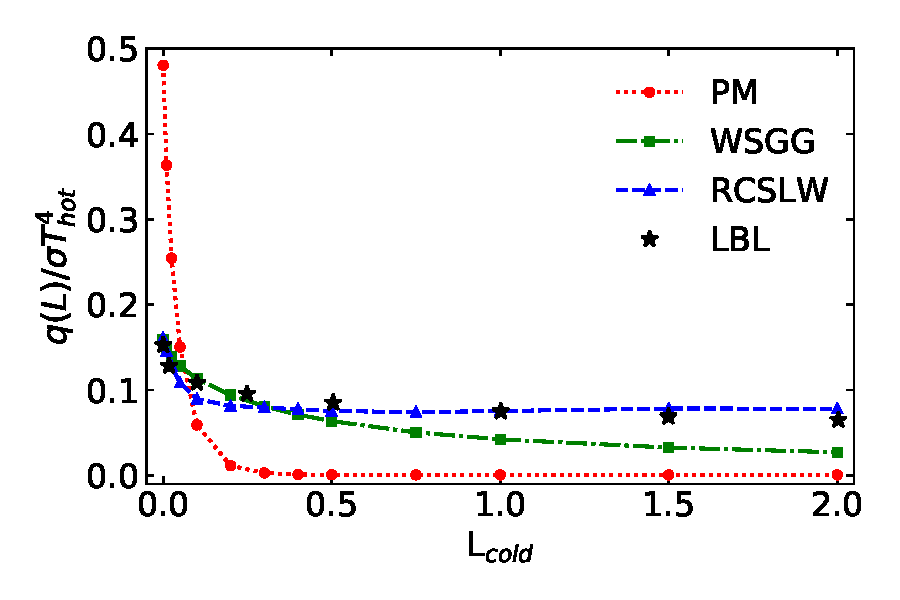
\includegraphics[width=2.75 in]{fig_ex_1.pdf} &
        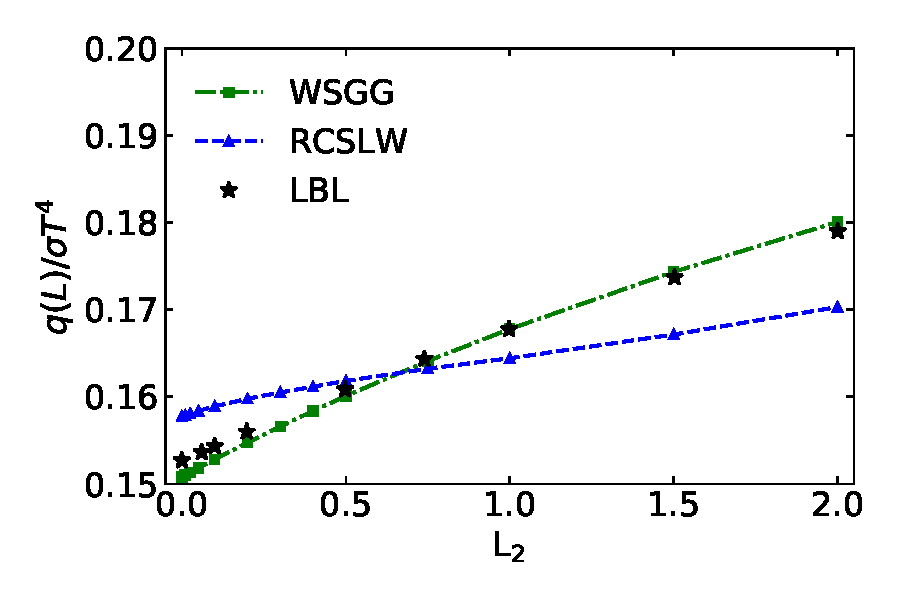
\includegraphics[width=2.75 in]{fig_ex_2b.pdf} \\
        Example S3 & Example S4 \\
        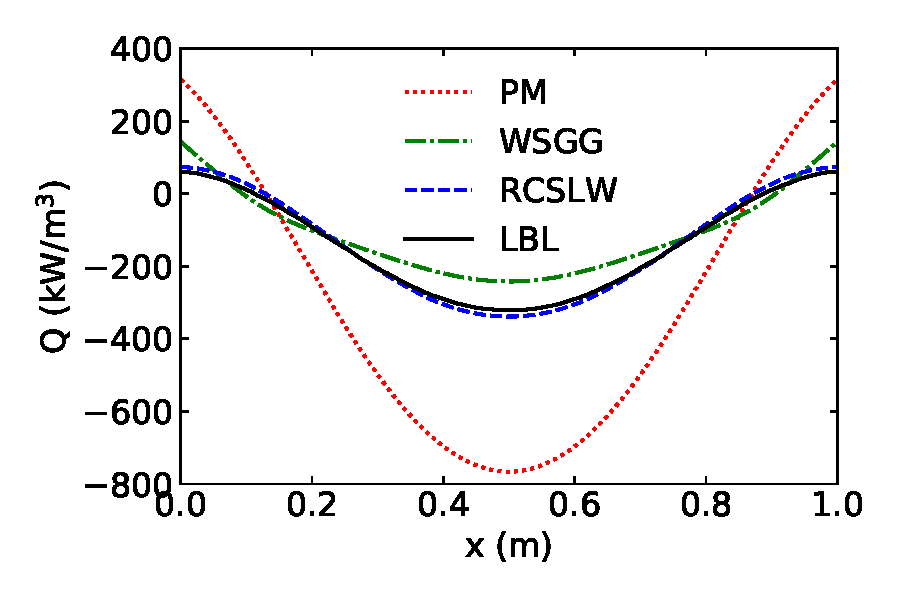
\includegraphics[width=2.75 in]{fig_ex_3a.pdf} &
        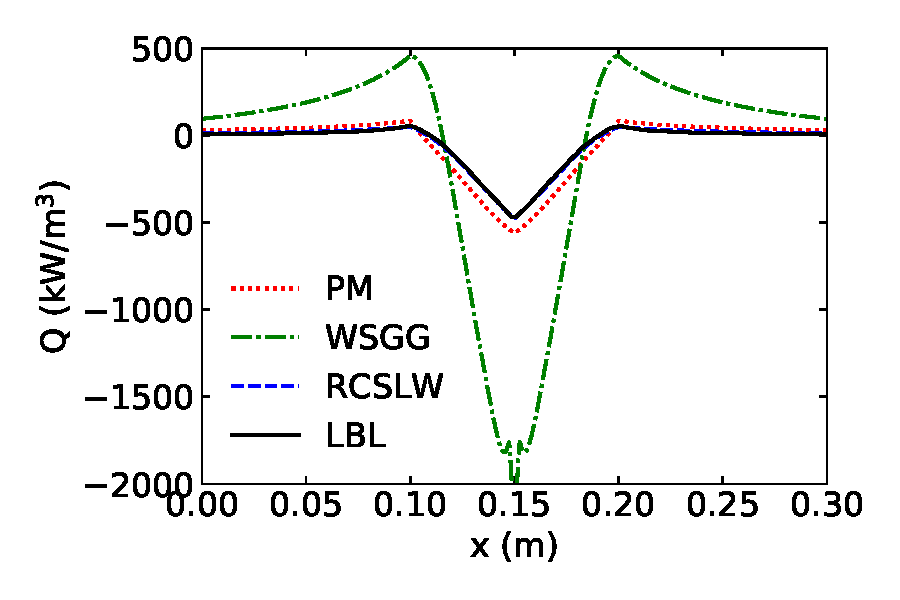
\includegraphics[width=2.75 in]{fig_ex_4a.pdf} \\
        Example S5 & Example B3 \\
        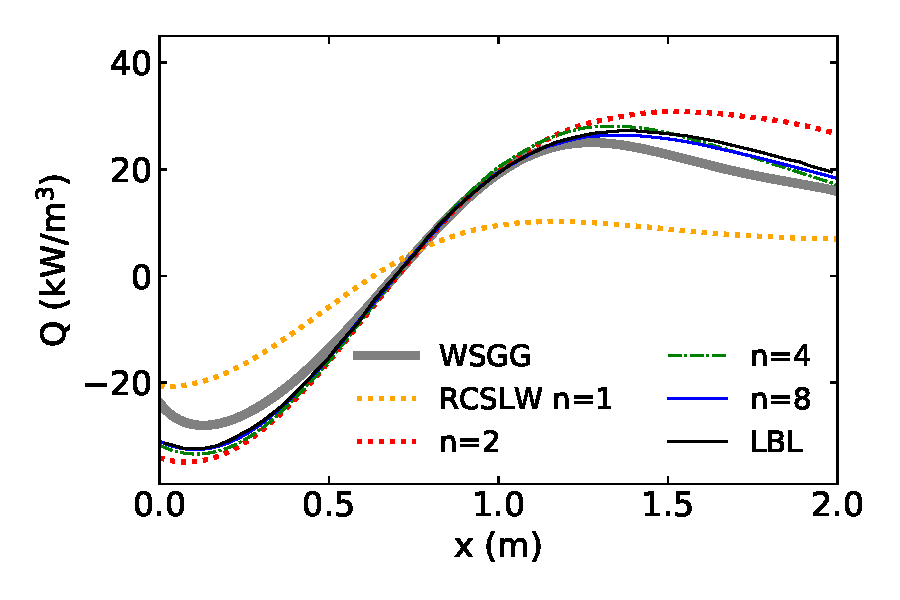
\includegraphics[width=2.75 in]{fig_ex_5b.pdf} &
        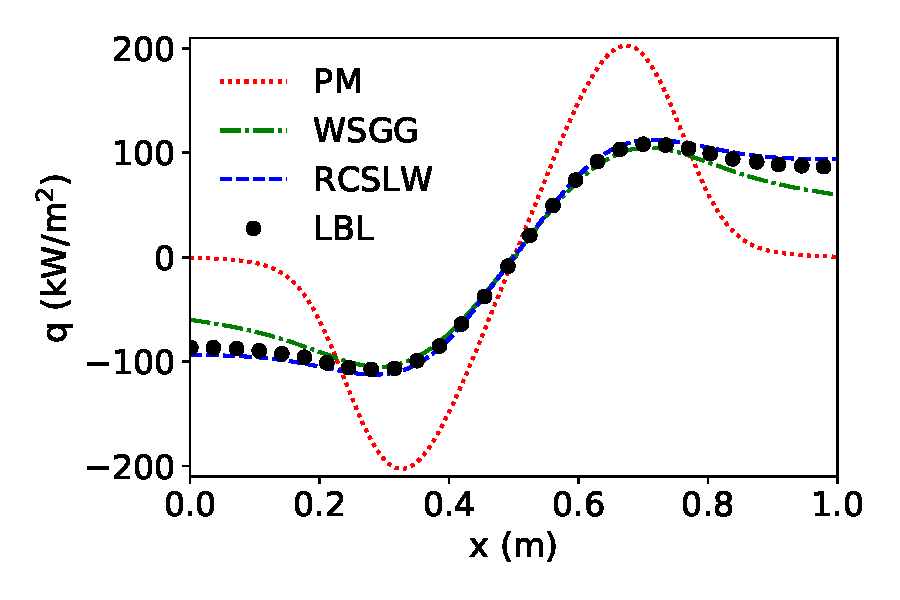
\includegraphics[width=2.75 in]{fig_ex_6.pdf}
    \end{tabular}
    \caption{Results for examples summarized in Table~\ref{t:examples}.}
    \label{f:examples}
    \end{center}
\end{figure}
%
In general, the PM model performs poorly compared to the WSSGG and RCSLW models. A notable exception is Example S4. In Example S2, the PM $q(L)/\sigma T^4$ is off scale at an essentially constant at a value of unity. The PM absorption coefficient is 27.4 atm$^{-1}$m$^{-1}$, giving optical thicknesses of 0.09 and 0.36 m in the thick and thin layers, respectively, which are relatively small compared to the isothermal domain size greater than 0.5 m. Example S5 omits the PM model to more clearly show the behavior of the WSGG and RCSLW models. For that example, the PM values follow the shape of the other curves but $Q$ varies from around -80 at $x=0$ to a peak of 200 at x=$1.5$ m, and dropping to 100 kW/m$^3$ at $x=2$ m. In all examples, four gray ($n=4$) and one clear gas are computed for the RCSLW models to give a consistent comparison to the WSGG model. Example S5 shows the sensitivity of the RCSLW model to the number of gases used. The difference between $n=2$ and $n=8$ is very small for all examples shwon, except for Example S2. When $n$ is increased from four to eight for that example the RCSLW model improves to show nearly perfect agreement with the LBL data.
In all Examples, the RCSLW model is initialized using the mean temperature and composition on the domain. In Example S5, the RCSLW model converges to the LBL solution when the model is initialized using the maximum temperature instead of the average temperature.

Figure~\ref{f:exSb1} shows the results from Example Sb1, which includes soot radiation. Results for three values of the soot volume fraction are shown. Both the WSGG and RCSLW models perform very well for each case. 
%
\begin{figure}
    \begin{center}
        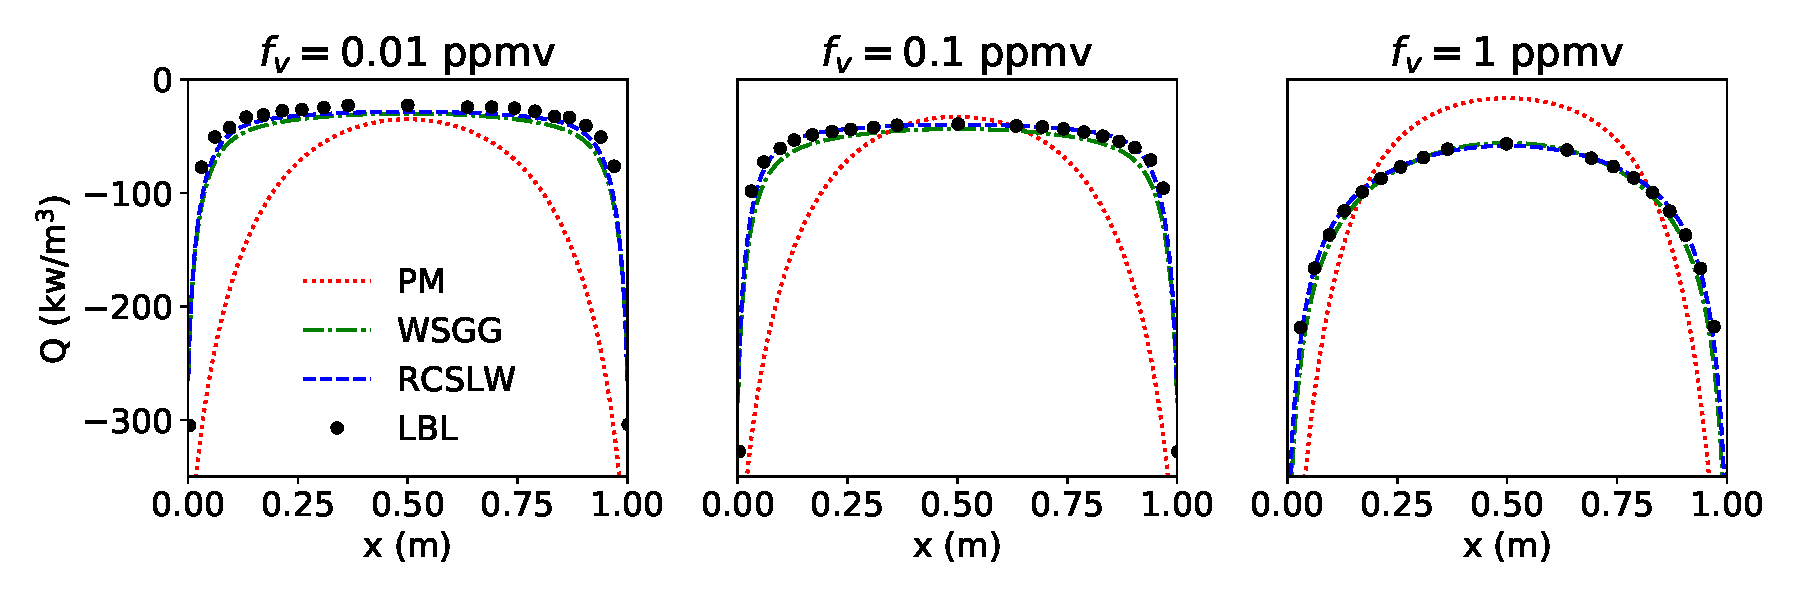
\includegraphics[width=5.5 in]{fig_ex_Sb1.pdf}
    \caption{Results for Example Sb1 summarized in Table~\ref{t:examples}.}
    \label{f:exSb1}
    \end{center}
\end{figure}
%

%%%%%%%%%%%%%%%%%%%%%%%%%%%%%%%%%%%%%%%%%%%%%%%%%%%%%%%%%%%%%%%%%%%%%%%%%%%%%%%%

\subsection{Computational Cost} \label{s:cost}

A comparison was made of the computational cost of the current models implemented. Calculations were performed on a 4 GHz Quad Core Intel Core i7 iMac, version 10.15.7. Figure~\ref{f:cost}a shows the cost to compute the gas properties $k$ and $a$. This was done by timing the C++ code execution to evaluate the gas properties one million times in a loop and then averaging the results. The figure shows times normalized by the time for the WSGG model, which required 8.0E-7~s. The costs of the models, relative to WSGG, is 0.098, 1.9, 4.9, 9.4, and 18, for PM, and RCSLW with $n=1$, 2, 4, 8 gray gases, respectively. The cost of the RCSLW model is very nearly proportional to the number of gray gases considered.
%
\begin{figure}
    \begin{center}
    \begin{tabular}{c c}
        (a) & (b) \\
        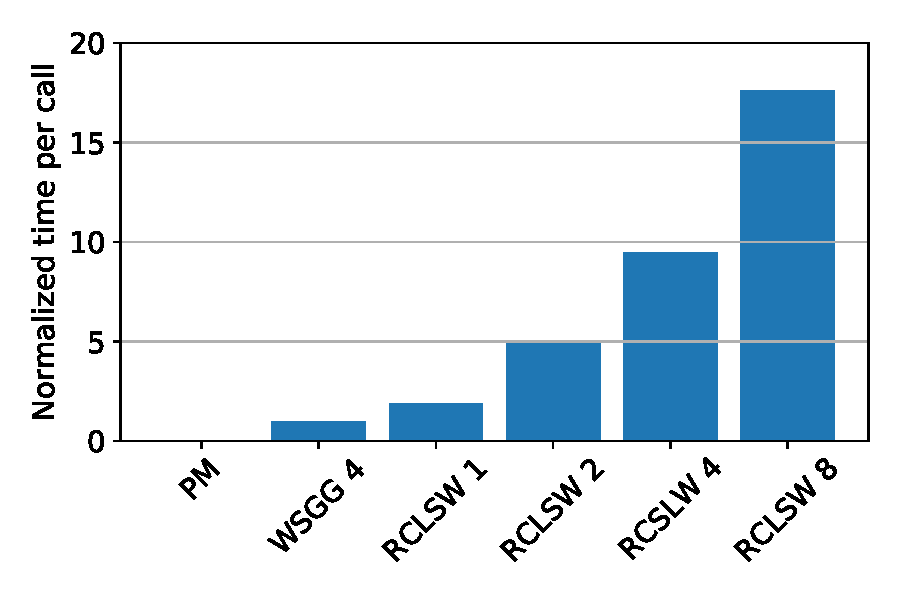
\includegraphics[width=2.75 in]{fig_getka_c++.pdf} &
        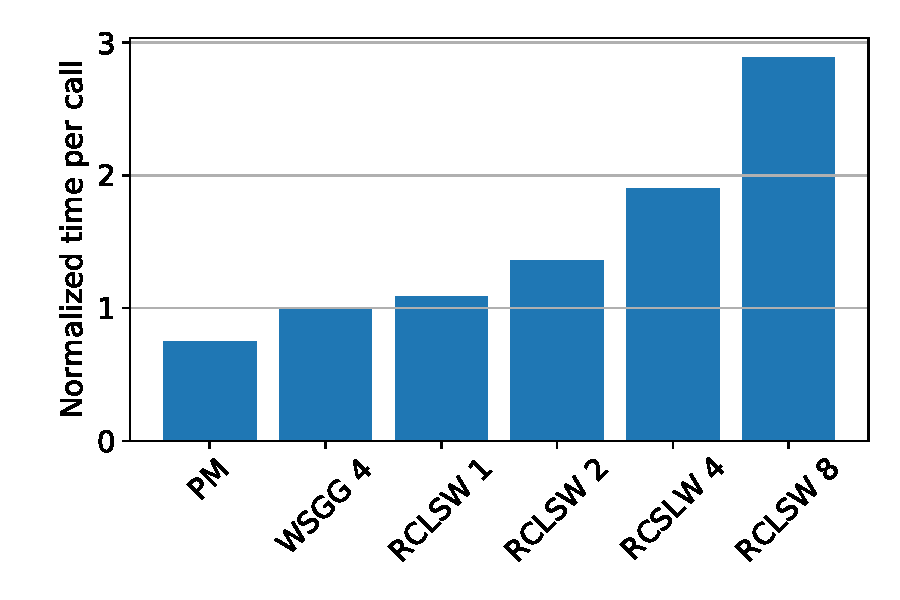
\includegraphics[width=2.75 in]{fig_exS3_c++.pdf}
    \end{tabular}
    \caption{Computational cost to evaluate gas properties (a) and to run Example S3 (b). Results are normalized by the cost of the WSSG model.}
    \label{f:cost}
    \end{center}
\end{figure}
%

Figure~\ref{f:cost}b shows the cost to evaluate Example S3. 
In this case the costs of the models, relative to WSGG, is approximately 0.75, 1.1, 1.4, 1.9, and 2.9, for PM, and RCSLW with $n=1$, 2, 4, 8 gray gases, respectively. Here, the WSGG model took 0.0079 s. In running Example S3, the costs of the various models are much more similar than in evaluating gas properties alone due to the additional overhead required in performing the calculations. In the results presented, only the cost of evaluating the solution was included; initialization and input/output costs were neglected.

Cost comparisons were also attempted with Python, but it is difficult to get meaningful results when mixing Python and C++. In particular, the cost of a single evaluation of the gas properties is small and evaluating the gas properties in a Python loop results in the loop appearing to dominate the computational cost. Comparison between Python and C++ for Example S3 is somewhat more meaningful, but even here, for the six cases considered in Fig.~\ref{f:cost} the cost only varied by about 4\%, indicating that the costs are dominated by the Python and not by the model calculations themselves. The cost of the WSGG model was 0.6~s, which is 7.6 times slower than the C++ version. It is possible that improvements to the Python speed could be made by further optimization of the Cython interface, but the Python radiative solver used in the examples is only meant to demonstrate the use of the library evaluation of gas properties.

%%%%%%%%%%%%%%%%%%%%%%%%%%%%%%%%%%%%%%%%%%%%%%%%%%%%%%%%%%%%%%%%%%%%%%%%%%%%%%%%

\section{Discussion} \label{s:impact}

Radiative heat transfer models are historically difficult to implement in CFD codes due to their complexity and high computational costs. Neglecting radiation or using simple models like the optically thin assumption is adequate for some cases with simple geometry or limited chemical reactions, but most simulations of interest to engineers and researchers require more advanced radiation modeling to yield accurate results. In such cases, radiation models that are incorrectly implemented or inappropriate for the simulation parameters can become additional sources of error that may be extremely difficult to separate from existing sources or error. Currently, researchers that require detailed radiation modeling must code and validate it themselves at the expense of valuable research time and funding. 

RadLib makes researchers' work easier by consolidating various approaches into a modular library of interchangeable, prevalidated radiation models. Additionally, RadLib's modular framework is designed to easily accommodate new models as well, allowing researchers to compare new or existing models with very little overhead. Sometimes, it is not clear which radiation model may be the best fit for a particular simulation. When simulations are especially complex or computationally expensive, researchers may have to extrapolate from theory and literature to choose an appropriate radiation model rather than testing for their specific case. RadLib is designed to ease both of these obstacles by facilitating comparison between radiation models through a common interface and providing a practical means of testing various models without the restriction of prespecified geometry or case parameters. With RadLib, researchers can put more of their time and effort into useful results rather than code or model development. 

Currently, RadLib is only used within the authors' research group, where it is applied to combustion CFD simulations using the One-Dimensional Turbulence (ODT) model \cite{Stephens_2020}, but its design and structure as a C++ library allows it to be incorporated easily into existing codes. It can be applied to  research questions in various other fields involving radiative heat transfer as well, including energy engineering or atmospheric and climate sciences. Radiation is a universal phenomenon, and RadLib can assist researchers in many areas with systems and processes that involve heat transfer. 

%Author guidelines for this section
%\begin{itemize}
% \item \textbf{This is the main section of the article and the reviewers weight the description here appropriately}
% \item Indicate in what way new research questions can be pursued as a result of the software (if any).
% \item Indicate in what way, and to what extent, the pursuit of existing research questions is improved (if so).
% \item Indicate in what way the software has changed the daily practice of its users (if so).
% \item Indicate how widespread the use of the software is within and outside the intended user group.
% \item Indicate in what way the software is used in commercial settings and/or how it led to the creation of spin-off companies (if so).
%\end{itemize}

%%%%%%%%%%%%%%%%%%%%%%%%%%%%%%%%%%%%%%%%%%%%%%%%%%%%%%%%%%%%%%%%%%%%%%%%%%%%%%%%

\section{Conclusions} \label{s:conclusions}

RadLib is a C++ library of radiation property models developed to address the complexity and difficulty inherent in implementing radiative property models in CFD simulations. At present, it includes three major radiation property models---Planck Mean (PM) absorption coefficients, the weighted sum of gray gases (WSGG) model, and the rank-correlation spectral line weighted-sum-of-gray-gases (RCSLW) model---but its modular design and C++ and Python interfaces permit convenient expansion to additional property models. To that end, the basic structure and use of the RadLib library has been laid out. In addition, the RadLib package includes example cases in several variations of a parallel planes geometry using a simple ray tracing solver to illustrate the use of the three radiation property models. These examples are compared to line-by-line solutions. In general, the RCSLW model outperforms both the PM and WSGG models in terms of accuracy, but, under the appropriate conditions, the PM and WSGG models can also perform well and boast lower computational costs than the RCSLW model. As a whole, RadLib provides a convenient access point for researchers that require radiation property models for simulation tools and can be applied to research problems in a variety of fields. 

%%%%%%%%%%%%%%%%%%%%%%%%%%%%%%%%%%%%%%%%%%%%%%%%%%%%%%%%%%%%%%%%%%%%%%%%%%%%%%%%

\section{Declaration of Competing Interes} \label{s:coi}

The authors declare that they have no known competing financial interests or personal relationships that could have appeared to influence the work reported in this paper.


%%%%%%%%%%%%%%%%%%%%%%%%%%%%%%%%%%%%%%%%%%%%%%%%%%%%%%%%%%%%%%%%%%%%%%%%%%%%%%%%

\section*{Acknowledgements} \label{sec:acknowledgements}

The authors extend special thanks to Hadi Bordbar for assistance with the WSGG model and to Vladimir Solovjov and Brent Webb for their insights and assistance with the RCSLW model. 
This research did not receive any specific grant from funding agencies in the public, commercial, or
not-for-profit sectors.

%%%%%%%%%%%%%%%%%%%%%%%%%%%%%%%%%%%%%%%%%%%%%%%%%%%%%%%%%%%%%%%%%%%%%%%%%%%%%%%%

%\bibliographystyle{elsarticle-num} 
%\bibliography{references} 

\begin{thebibliography}{10}
\expandafter\ifx\csname url\endcsname\relax
  \def\url#1{\texttt{#1}}\fi
\expandafter\ifx\csname urlprefix\endcsname\relax\def\urlprefix{URL }\fi
\expandafter\ifx\csname href\endcsname\relax
  \def\href#1#2{#2} \def\path#1{#1}\fi

\bibitem{Hottel_1967}
H.~Hottel, A.~Sarofim, Radiative Transfer, {McGraw-Hill}, New York, 1967.

\bibitem{Modest_2013}
M.~F. Modest, Radiative Heat Transfer, third edition Edition, {Academic Press},
  New York, 2013.

\bibitem{Smith_2003}
N.~Smith, J.~Gore, J.~Kim, Q.~Tang,
  \href{https://tnfworkshop.org/radiation/}{{TNF} workshop radiation models}
  (2003).
\newline\urlprefix\url{https://tnfworkshop.org/radiation/}

\bibitem{Grosshandler_1993}
W.~L. Grosshandler, {RADCAL}: A narrow-band model for radiation calculations in
  a combustion environment: Nist technical note 1402.

\bibitem{Barlow_2001}
R.~S. Barlow, A.~N. Karpetis, J.~H. Frank, J.-Y. Chen, Scalar profiles and {NO}
  formation in laminar opposed-flow partially premixed methane/air flames,
  Combustion and Flame 127~(3) (2001) 2102--2118.
\newblock \href {http://dx.doi.org/10.1016/S0010-2180(01)00313-3}
  {\path{doi:10.1016/S0010-2180(01)00313-3}}.

\bibitem{Barlow_1999}
R.~Barlow, N.~Smith, J.~Chen, R.~Bilger,
  \href{http://www.sciencedirect.com/science/article/pii/S0010218098000716}{Nitric
  oxide formation in dilute hydrogen jet flames: isolation of the effects of
  radiation and turbulence-chemistry submodels}, Combustion and Flame 117~(1-2)
  (1999) 4--31.
\newblock \href {http://dx.doi.org/10.1016/S0010-2180(98)00071-6}
  {\path{doi:10.1016/S0010-2180(98)00071-6}}.
\newline\urlprefix\url{http://www.sciencedirect.com/science/article/pii/S0010218098000716}

\bibitem{Frank_2000}
J.~H. Frank, R.~S. Barlow, C.~Lundquist, Radiation and nitric oxide formation
  in turbulent non-premixed jet flames, Proceedings of the Combustion Institute
  28~(1) (2000) 447--454.
\newblock \href {http://dx.doi.org/10.1016/S0082-0784(00)80242-8}
  {\path{doi:10.1016/S0082-0784(00)80242-8}}.

\bibitem{Zhu_2002}
X.~Zhu, J.~Gore, A.~N. Karpetis, R.~S. Barlow,
  \href{http://www.sciencedirect.com/science/article/pii/S0010218002003413}{The
  effects of self-absorption of radiation on an opposed flow partially premixed
  flame}, Combustion and Flame 129~(3) (2002) 342--345.
\newblock \href {http://dx.doi.org/10.1016/S0010-2180(02)00341-3}
  {\path{doi:10.1016/S0010-2180(02)00341-3}}.
\newline\urlprefix\url{http://www.sciencedirect.com/science/article/pii/S0010218002003413}

\bibitem{Coelho_2002}
P.~J. Coelho, O.~J. Teerling, D.~Roekaerts, Spectral radiative effects and
  turbulence-radiation-interaction in sandia flame {D}, in: {Barlow, Robert S.,
  Pope, Stephan B., Masri, Assaad R., Oefelein, Joseph C.} (Ed.), The
  Proceedings of the Sixth International Workshop on Measurement and
  Computation of Turbulent Nonpremixed Flames, 2002.

\bibitem{Bordbar_2014}
M.~H. Bordbar, G.~Wecel, T.~Hyppanen, A line by line based weighted sum of gray
  gases model for inhomogeneous {CO$_2$–H$_2$O} mixture in oxy-fired
  combustion, Combustion and Flame 161~(9) (2014) 2435--2445.
\newblock \href {http://dx.doi.org/10.1016/j.combustflame.2014.03.013}
  {\path{doi:10.1016/j.combustflame.2014.03.013}}.

\bibitem{Bordbar_2020}
H.~Bordbar, G.~C. Fraga, S.~Hostikka,
  \href{http://www.sciencedirect.com/science/article/pii/S0735193319302660}{An
  extended weighted-sum-of-gray-gases model to account for all {CO$_2$-H$_2$O}
  molar fraction ratios in thermal radiation}, International Communications in
  Heat and Mass Transfer 110 (2020) 104400.
\newblock \href {http://dx.doi.org/10.1016/j.icheatmasstransfer.2019.104400}
  {\path{doi:10.1016/j.icheatmasstransfer.2019.104400}}.
\newline\urlprefix\url{http://www.sciencedirect.com/science/article/pii/S0735193319302660}

\bibitem{Rothman_2010}
L.~S. Rothman, I.~E. Gordon, R.~J. Barber, H.~Dothe, R.~R. Gamache, A.~Goldman,
  V.~I. Perevalov, S.~A. Tashkun, J.~Tennyson,
  \href{http://www.sciencedirect.com/science/article/pii/S002240731000169X}{{HITEMP},
  the high-temperature molecular spectroscopic database}, Journal of
  Quantitative Spectroscopy {\&} Radiative Transfer 111~(15) (2010) 2139--2150.
\newblock \href {http://dx.doi.org/10.1016/j.jqsrt.2010.05.001}
  {\path{doi:10.1016/j.jqsrt.2010.05.001}}.
\newline\urlprefix\url{http://www.sciencedirect.com/science/article/pii/S002240731000169X}

\bibitem{Solovjov_2016}
V.~P. Solovjov, F.~Andr{\'e}, D.~Lemonnier, B.~W. Webb, The generalized {SLW}
  model, Journal of Physics: Conference Series 676 (2016) 1--36.

\bibitem{Solovjov_2017}
V.~P. Solovjov, F.~Andr{\'e}, D.~Lemonnier, B.~W. Webb, The rank correlated
  {SLW} model of gas radiation in non-uniform media, Journal of Quantitative
  Spectroscopy {\&} Radiative Transfer 197 (2017) 26--44.
\newblock \href {http://dx.doi.org/10.1016/j.jqsrt.2017.01.034}
  {\path{doi:10.1016/j.jqsrt.2017.01.034}}.

\bibitem{Badger_2019}
J.~Badger, B.~W. Webb, V.~P. Solovjov, An exploration of advanced {SLW}
  modeling approaches in comprehensive combustion predictions, Combustion
  Science and Technology 012022~(676) (2019) 1--17.
\newblock \href {http://dx.doi.org/10.1080/00102202.2019.1678907}
  {\path{doi:10.1080/00102202.2019.1678907}}.

\bibitem{Solovjov_2000}
V.~P. Solovjov, B.~W. Webb, {SLW} modeling of radiative transfer in
  multicomponent gas mixtures, Journal of Quantitative Spectroscopy and
  Radiative Transfer 65 (2000) 655--672.

\bibitem{Solovjov_2001}
V.~P. Solovjov, B.~W. Webb, An efficient method for modeling radiative transfer
  in multicomponent gas mixtures with soot, Transactions of the ASME 123 (2001)
  450--457.

\bibitem{Solovjov_2008}
V.~P. Solovjov, B.~W. Webb, Multilayer modeling of radiative transfer by {SLW}
  and {CW} methods in non-isothermal gaseous medium, Journal of Quantitative
  Spectroscopy and Radiative Transfer 109~(2) (2008) 245--257.
\newblock \href {http://dx.doi.org/10.1016/j.jqsrt.2007.08.015}
  {\path{doi:10.1016/j.jqsrt.2007.08.015}}.

\bibitem{Solovjov_2011}
V.~P. Solovjov, D.~Lemonnier, B.~W. Webb, The {SLW}-1 model for efficient
  prediction of radiative transfer in high temperature gases, Journal of
  Quantitative Spectroscopy and Radiative Transfer 112~(7) (2011) 1205--1212.
\newblock \href {http://dx.doi.org/10.1016/j.jqsrt.2010.08.009}
  {\path{doi:10.1016/j.jqsrt.2010.08.009}}.

\bibitem{Solovjov_2014}
V.~P. Solovjov, D.~Lemonnier, B.~W. Webb, Extension of the exact {SLW} model to
  non-isothermal gaseous media, Journal of Quantitative Spectroscopy and
  Radiative Transfer 143 (2014) 83--91.
\newblock \href {http://dx.doi.org/10.1016/j.jqsrt.2013.10.008}
  {\path{doi:10.1016/j.jqsrt.2013.10.008}}.

\bibitem{Webb_2018}
B.~W. Webb, V.~P. Solovjov, F.~Andr{\'e}, An exploration of the influence of
  spectral model parameters on the accuracy of the rank correlated slw model,
  Journal of Quantitative Spectroscopy and Radiative Transfer 218 (2018)
  161--170.
\newblock \href {http://dx.doi.org/10.1016/j.jqsrt.2018.06.023}
  {\path{doi:10.1016/j.jqsrt.2018.06.023}}.

\bibitem{Pearson_2014}
J.~Pearson, B.~Webb, S.~V.P., J.~Ma, Efficient representation of the absorption
  line blackbody distribution function for {H$_2$O}, {CO$_2$}, and {CO} at
  variable temperature, mole fraction, and total pressure, Journal of
  Quantitative Spectrosopy and Radiative Transfer 138 (2014) 82--96.

\bibitem{Brewster_1992}
M.~Q. Brewster, Thermal Radiative Transfer and Properties, Wiley, 1992.

\bibitem{Lee_1981}
S.~C. Lee, C.~L. Tien, Optical constants of soot in hydrocarbon flames,
  Symposium (International) on Combustion 18~(1) (1981) 1159--1166.
\newblock \href {http://dx.doi.org/10.1016/S0082-0784(81)80120-8}
  {\path{doi:10.1016/S0082-0784(81)80120-8}}.

\bibitem{Stull_1960}
V.~R. Stull, G.~N. Plass, Emissivity of dispersed carbon particles, Journal of
  the Optical Society of America 50~(2) (1960) 121.
\newblock \href {http://dx.doi.org/10.1364/JOSA.50.000121}
  {\path{doi:10.1364/JOSA.50.000121}}.

\bibitem{Dalzell_1969}
W.~H. Dalzell, A.~F. Sarofim, Optical constants of soot and their application
  to heat-flux calculations, Journal of Heat Transfer 91~(1) (1969) 100--104.
\newblock \href {http://dx.doi.org/10.1115/1.3580063}
  {\path{doi:10.1115/1.3580063}}.

\bibitem{Howarth_1966}
C.~R. Howarth, P.~J. Foster, M.~W. Thring (Eds.), The Effect of Temperature on
  the Extinction of Radiation By Soot Particles, Begellhouse, 1966.
\newblock \href {http://dx.doi.org/10.1615/IHTC3.1210}
  {\path{doi:10.1615/IHTC3.1210}}.

\bibitem{Chang_1990}
H.-c. Chang, T.~T. Charalampopoulos, Determination of the wavelength dependence
  of refractive indices of flame soot, Proceedings of the Royal Society of
  London. Series A: Mathematical and Physical Sciences 430~(1880) (1990)
  577--591.
\newblock \href {http://dx.doi.org/10.1098/rspa.1990.0107}
  {\path{doi:10.1098/rspa.1990.0107}}.

\bibitem{Felske_1984}
J.~D. Felske, T.~T. Charalampopoulos, H.~S. Hura, Determination of the
  refractive indices of soot particles from the reflectivities of compressed
  soot pellets, Combustion Science and Technology 37~(5-6) (1984) 263--283.
\newblock \href {http://dx.doi.org/10.1080/00102208408923757}
  {\path{doi:10.1080/00102208408923757}}.

\bibitem{Williams_2007}
T.~C. Williams, C.~R. Shaddix, K.~A. Jensen, J.~M. Suo-Anttila, Measurement of
  the dimensionless extinction coefficient of soot within laminar diffusion
  flames, International Journal of Heat and Mass Transfer 50~(7-8) (2007)
  1616--1630.
\newblock \href {http://dx.doi.org/10.1016/j.ijheatmasstransfer.2006.08.024}
  {\path{doi:10.1016/j.ijheatmasstransfer.2006.08.024}}.

\bibitem{Felske_1977}
J.~Felske, T.~C.L., The use of the {M}ilne-{E}ddington absorption coefficient
  for radiative heat transfer in combustion systems, ASME Journal of Heat
  Transfer 99~(3) (1977) 633--647.

\bibitem{Bordbar_personal}
H.~Bordbar, personal communication.

\bibitem{Chang_1984}
S.~Chang, K.~Rhee, Blackbody radiation functions, International communictions
  in Heat and Mass Transfer 11 (1984) 451--455.

\bibitem{Stephens_2020}
V.~Stephens, D.~Lignell, One-dimensional turbulence ({ODT}): computationally
  efficient modeling and simulation of turbulent flows, Software{X} 13 (2020)
  100641.
\newblock \href {http://dx.doi.org/10.1016/j.softx.2020.100641}
  {\path{doi:10.1016/j.softx.2020.100641}}.

\end{thebibliography}

%%%%%%%%%%%%%%%%%%%%%%%%%%%%%%%%%%%%%%%%%%%%%%%%%%%%%%%%%%%%%%%%%%%%%%%%%%%%%%%%

\end{document}
\endinput

